\documentclass{article}
\usepackage{graphicx} % Required for inserting images
\usepackage{subcaption}
\usepackage[T2A]{fontenc}
\usepackage[ruled,vlined]{algorithm2e}

\title{Роевой алгоритм для задачи TSP}
\author{Добрыня Меркурьев}
\date{April 2026}

\begin{document}

\maketitle

\begin{abstract}
    В данном проекте рассматривается решение задачи коммивояжера (TSP --- Traveling Salesman Problem) при помощи метода муравьиной колонии (ACO --- Ant Colony Optimization). Исследуются различные стратегии выбора пути и распределения феромона, сравнивается их эффективность относительно трудозатратности.
\end{abstract}

\section{Введение}
Задача коммивояжера (TSP) заключается в нахождении гамильтонова цикла с наименьшим суммарным весом ребер в полном взвешенном графе. Задача называется симметричной, если вес ребра равен весу обратного, геометрической -- если вершины графа представимы на плоскости так, что веса ребер между соответствуют расстоянию между точками. Очевидно, что геометрическая задача симметрична. В практической части данной работы будет рассматриваться геометрическая вариация TSP, но все используемые алгоритмы могут быть применены к произвольной задаче коммивояжера с минимальными изменениями.

Метод муравьиной колонии (ACO) это метаэвристика для комбинаторных задач оптимизации, в которой задача решается муравьями, пошагово строящими решение. Они применимы к любой задаче оптимизации, на которой можно определить эвристику для частичного решения, но впервые этот метод был использован в алгоритме Ant System для решения TSP. \cite{AS} Даже во время публикации этот метод не превосходил лучшие методы решения TSP, поэтому вскоре были предложены различные модификации алгоритма Ant System, улучшающие его эффективность.


\section{Теория}
\subsection{Формальные определения}

Задачей оптимизации называют $\Bigl(x, F(x), c(s)\Bigr)$, где $x$ --- экземпляр задачи, $F(x)$ --- множество корректных решений, $c(s), s \in F(x)$ --- цена решения. Решение задачи оптимизации --- это наименьшее (наибольшее) по стоимости решение $OPT(x)=\min_{s\in F(x)} c(s)$ (для наибольшего определяется аналогично). В случае TSP $x$ это матрица смежности, $F(x)$ --- все гамильтоновы циклы (можно представить как перестановки $1...n$), $c(s)$ --- суммарный вес ребер в цикле. 

Метаэвристика Ant Colony Optimization (ACO) это класс вероятностных алгоритмов, решающих задачу оптимизации пошагово собирая решение из некоторых элементов. На каждом шаге следующий элемент решения выбирается вероятностно относительно функции стоимости от частичного решения и значения феромона соответствующего этому переходу.

\subsection{Алгоритмы}
\subsubsection{Ant System}
Алгоритм Ant System представляет собой простейший вариант ACO и состоит из двух повторяющихся фаз --- построения пути муравьями и обновления феромона.

Каждый муравей начинает строить решение со случайной вершины графа. Он случайно выбирает следующий пункт маршрута на основе весов ребер и феромоне на них. Если вес ребра в $i$-ю вершину из текущей -- $w_{i}$, а количество феромона на нем -- $p_{i}$, то вероятность перехода муравья по этому ребру равна 
\[ P=\frac{p_i^\alpha w_i^\beta}{S}, S=\sum_{j=1}^{n} p_j^\alpha w_j^\beta I_j \]
где $\alpha$ и $\beta$ ---- некоторые суперпараметры алгоритма, а $I_j$ --- индикатор того, что муравей еще не посетил вершину $j$.

После того, как все муравьи построят пути, они замыкаются до цикла и происходит перерасчет феромона. Сначала часть феромона испарится (это нужно для того, чтобы система могла "забывать" старые решения в пользу более оптимальных), а затем каждый муравей оставит феромон на своем пути в обратно пропорциональном длине его пути количестве.
\[p_i^{new}=p_i(1-\rho)+\sum_{k\in K_i}\frac1{C_k}\]
где $K_i$ множество номеров муравьев, чей путь проходит через $i$-е ребро, а $C_k$ --- суммарная длина пути $k$-го муравья, а $\rho\in[0;1]$ --- скорость испарения.

\subsubsection{Elitist Ant System}
Небольшая модификация AS, сдвигающая решение в сторону кратчайшего из уже найденных маршрутов. В дополнение к обычному распределению феромон будет вноситься по кратчайшему из найденных путей, независимо от того, проходили ли его муравьи в текущей итерации. Формула перерасчета феромона станет такой:
\[p_i^{new}=p_i(1-\rho)+\sum_{k\in K_i}\frac1{C_k}+\frac e {C_{best}}\]
где $e$ -- некоторая константа, а $C_{best}$ -- длина лучшего из найденных маршрутов.

\subsubsection{Max-Min Ant System}
Предложенная в \cite{MMAS} модификация AS, подталкивающая муравьев к большему исследованию возможных путей во первых ограниченем значений феромона на ребрах, а во вторых позволяя только лучшему муравью добавлять феромон. Таким образом, не случится стагнации --- случая, когда все муравьи идут одним маршрутом.

Изначально феромон устанавливается по верхней границе обрезается под границы после каждой итерации. В качестве вносящего вклад муравья можно выбирать как лучшего в итерации, так и глобально. Лучшие результаты в оригинальной статье были показаны на чередовании обоих вариантов.

\section{Практические результаты}
\subsection{Реализация}
Алгоритмы AS, EAS и MMAS были реализованы, используя описанные в \cite{4129846} оптимизации --- преподсчет весов выбора один раз вместо расчета заново для каждого муравья, массив посещенных муравьем вершин для быстрого поиска. Общая структура кода близка к показанной там.

Основной цикл алгоритма для n городов выглядит так:
\begin{algorithm}
\caption{Ant System}
Инициализировать феромон\;

\For{$iter = 1$ \KwTo $max\_iter$}{
    Построить веса выбора\;

    \ForEach{ant}{
        Разместить в случайном городе\;
    }

    \For{$i = 1$ \KwTo $n$}{
        \ForEach{ant}{
            Сделать случайный шаг\;
        }
    }

    Обновить феромон\;
}
\end{algorithm}

\begin{algorithm}
\caption{Обновить феромон}
\ForEach{edge}{
    edge.pheromone *= $1 - \rho$\;
}
Добавление феромона\;
\end{algorithm}

Конкретные алгоритмы отличаются методами инициализации и добавления феромона.
\newpage
\begin{algorithm}
\caption{Добавление феромона AS}
\ForEach{ant}{
    \For{edge $\in$ ant.path}{
        edge.pheromone += 1 / ant.path\_length\;
    }
}
\end{algorithm}

\begin{algorithm}
\caption{Добавление феромона EAS}
\ForEach{ant}{
    \For{edge $\in$ ant.path}{
        edge.pheromone += 1 / ant.path\_length\;
    }
}

\For{edge $\in$ best\_path}{
    edge.pheromone += e / best\_path.length\;
}
\end{algorithm}

\begin{algorithm}
\caption{Добавление феромона MMAS}
path := Случайно выбрать из best\_path и best\_iter\_path\;
\For{edge $\in$ path}{
    edge.pheromone += 1 / path.length\;
}

\For{edge $\in$ edges}{
    Ограничить edge.pheromone между $\tau_{min}$ и $\tau_{max}$\;
}
\end{algorithm}

В данной реализации вероятность выбора best\_path была 10\%.

\subsection{Результаты}
Все три алгоритма показали примерно одинаковое время на итерацию, несмотря на различное количество вносящих вклад муравьев. Это обусловлено тем, что основная масса вычислений приходится на построение путей, а не на добавление феромона.

\begin{figure}[h]
    \centering

    \begin{subfigure}{0.49\textwidth}
        \centering
        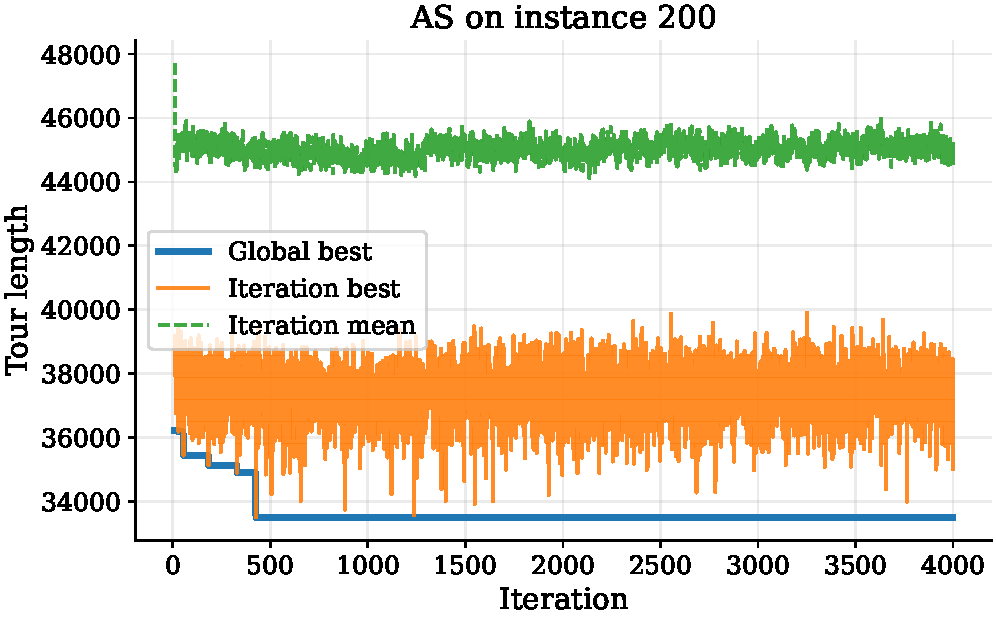
\includegraphics[width=\linewidth]{200_as_dynamics.pdf}
        \caption{Ant System}
    \end{subfigure}
    \begin{subfigure}{0.49\textwidth}
        \centering
        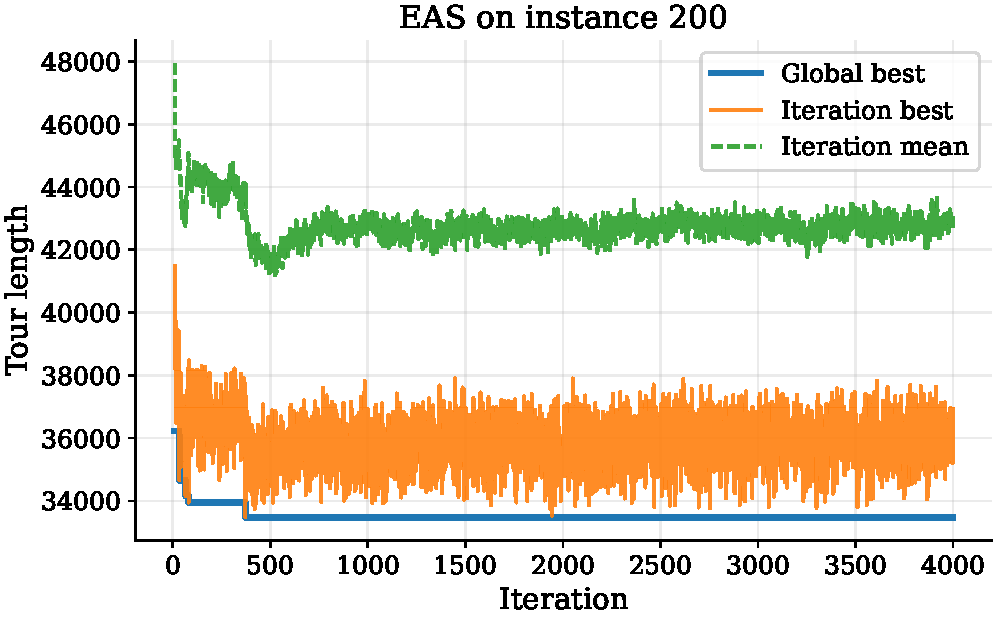
\includegraphics[width=\linewidth]{200_eas_dynamics.pdf}
        \caption{Elitist Ant System}
    \end{subfigure}
    \begin{subfigure}{0.49\textwidth}
        \centering
        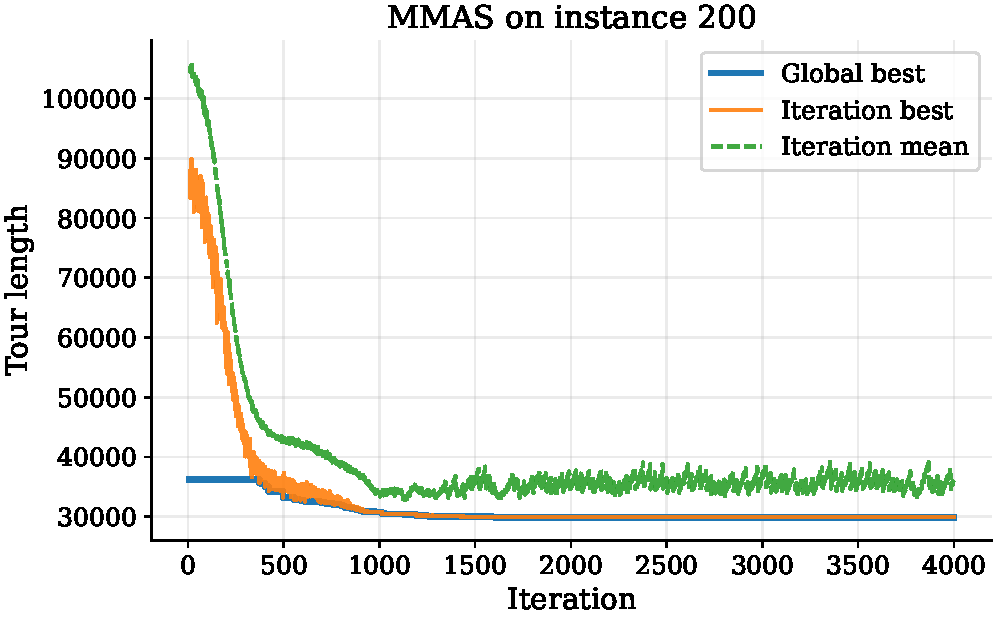
\includegraphics[width=\linewidth]{200_mmas_dynamics.pdf}
        \caption{Max-Min Ant System}
    \end{subfigure}
    \begin{subfigure}{0.49\textwidth}
        \centering
        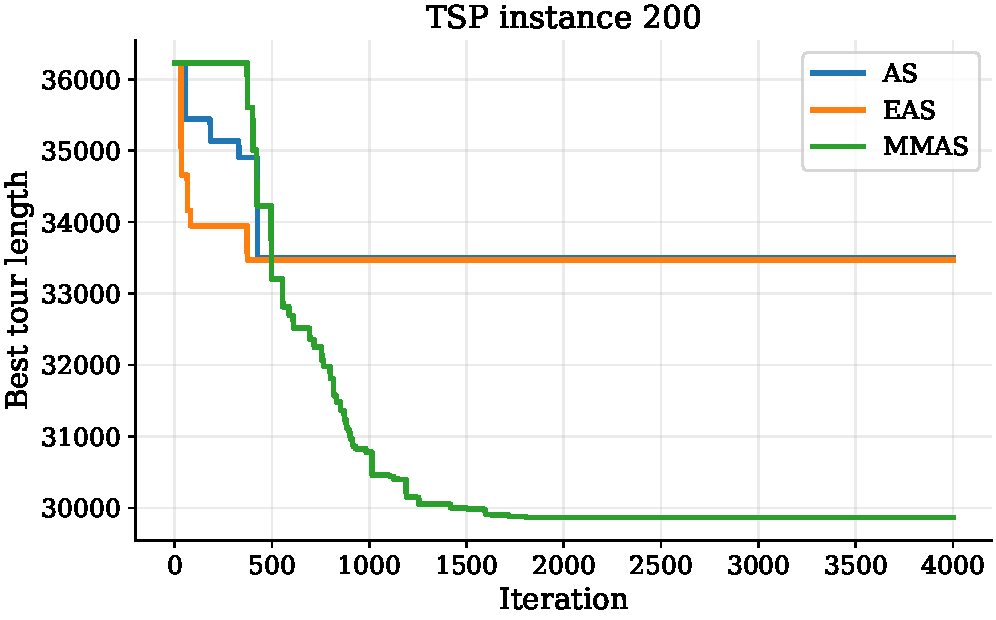
\includegraphics[width=\linewidth]{200_global_best.pdf}
        \caption{Лучшие решения}
    \end{subfigure}
    
    \caption{Динамика длины пути на разных алгоритмах}
    \label{fig:convergence_grid}
\end{figure}

Как видно из графиков, EAS концентрируется ближе к лучшему решению, за счет чего находит более короткие пути. MMAS начинает с гораздо более длинного решения, но показывает то, что авторы оригинальной статьи назвали сходимостью --- ребра, входящие в лучшее решение, имеют максимальное значение феромона, а остальные --- минимальное. Тем не менее, поиск решений продолжается, так как ограничения на феромон не дают системе выродиться в один единственный путь.

\bibliographystyle{plain}
\bibliography{refs}


\end{document}